\documentclass[tikz,border=10pt]{standalone}
\usepackage{tikz}
\usepackage{fontawesome5}
\usepackage{amsmath,amssymb}
\usetikzlibrary{arrows.meta,positioning,fit,backgrounds,calc,shadows,shapes.geometric}

% Color definitions
\definecolor{lavenderDark}{RGB}{15, 44, 89}
\definecolor{lavenderDeep}{RGB}{10, 28, 58}
\definecolor{lavenderMedium}{RGB}{29, 78, 158}
\definecolor{lavenderLight}{RGB}{240, 246, 255}
\definecolor{lavenderBorder}{RGB}{180, 205, 237}
\definecolor{prismNavy}{RGB}{15, 44, 89}
\definecolor{prismBlue}{RGB}{29, 78, 158}
\definecolor{prismTeal}{RGB}{13, 148, 136}
\definecolor{prismGold}{RGB}{217, 119, 6}
\definecolor{prismDark}{RGB}{15, 23, 42}
\definecolor{statusFail}{RGB}{220, 38, 38}
\definecolor{cInput}{RGB}{241, 245, 249}
\definecolor{cStem}{RGB}{224, 242, 254}
\definecolor{cStage1}{RGB}{209, 250, 229}
\definecolor{cStage2}{RGB}{254, 243, 199}
\definecolor{cHead}{RGB}{219, 234, 254}

\begin{document}
% Complete Flowchart for Blockchain Voting DApp & Double-Voting Mitigation
\begin{tikzpicture}[
  x=1cm, y=1cm,
  startend/.style={
    ellipse, draw=green!60!black, fill=green!45!black, text=white,
    line width=0.9pt, inner sep=3.5pt, font=\fontsize{7.5}{8.5}\selectfont\bfseries,
    minimum width=1.80cm, minimum height=0.60cm, drop shadow={opacity=0.12}
  },
  procbox/.style={
    rectangle, rounded corners=3.5pt,
    draw=lavenderDark!80, fill=white, text=black,
    line width=0.85pt, inner sep=4.0pt, font=\fontsize{7.0}{8.2}\selectfont,
    minimum height=0.75cm, text width=3.30cm, align=center, drop shadow={opacity=0.10}
  },
  decision/.style={
    diamond, aspect=2.0,
    draw=prismNavy, fill=lavenderLight, text=prismNavy,
    line width=0.85pt, inner sep=2.5pt, font=\fontsize{6.5}{7.6}\selectfont\bfseries,
    align=center, drop shadow={opacity=0.10}
  },
  errorbox/.style={
    rectangle, rounded corners=3pt,
    draw=statusFail!80, fill=statusFail!12, text=statusFail!90!black,
    line width=0.80pt, inner sep=3.5pt, font=\fontsize{6.5}{7.5}\selectfont\bfseries,
    minimum height=0.65cm, text width=2.40cm, align=center
  },
  flowarr/.style={
    -{Stealth[scale=0.85]}, line width=0.85pt, draw=lavenderDark!90
  },
  failarr/.style={
    -{Stealth[scale=0.80]}, line width=0.80pt, draw=statusFail!90, dashed
  }
]

  % Start
  \node[startend] (start) at (0, 0) {START};

  % Connect Wallet
  \node[procbox, fill=cInput, below=0.55cm of start] (connect) {
    \textbf{MetaMask Handshake}\\
    Request account access (\texttt{msg.sender})
  };

  % Decision 1: Is Admin?
  \node[decision, below=0.60cm of connect] (d_admin) {
    Is Caller\\Administrator?
  };

  % Admin Branch (Left)
  \node[procbox, fill=cStem, left=1.2cm of d_admin] (admin_portal) {
    \textbf{Admin Dashboard}\\
    Access \texttt{admin.html}
  };
  \node[procbox, fill=cHead, below=0.70cm of admin_portal] (admin_ops) {
    \textbf{Administrative Actions}\\
    $\bullet$ \texttt{addCandidate(name)}\\
    $\bullet$ \texttt{registerVoter(address)}
  };
  \node[procbox, fill=cStage1, below=0.70cm of admin_ops] (admin_commit) {
    \textbf{EVM State Update}\\
    Update candidate array /\\
    whitelist mapping
  };

  % Voter Branch: Check Registered
  \node[decision, below=0.75cm of d_admin] (d_reg) {
    Is Address\\Whitelisted?
  };
  \node[errorbox, right=1.2cm of d_reg] (err_reg) {
    \faTimesCircle\ REVERT:\\
    Unregistered Voter
  };

  % Voter Branch: Check Already Voted
  \node[decision, below=0.75cm of d_reg] (d_voted) {
    Has Address\\Already Voted?
  };
  \node[errorbox, right=1.2cm of d_voted] (err_voted) {
    \faBan\ REVERT:\\
    Double Vote Rejected
  };

  % Ballot Casting
  \node[procbox, fill=cStem, below=0.75cm of d_voted] (ballot_view) {
    \textbf{Display Ballot Portal}\\
    Show certified candidate list
  };
  \node[procbox, fill=cStage2, below=0.55cm of ballot_view] (sign_tx) {
    \textbf{Sign Ballot Transaction}\\
    Voter confirms candidate $c$ in MetaMask
  };
  \node[procbox, fill=cStage1, below=0.55cm of sign_tx] (atomic_evm) {
    \textbf{Atomic EVM Execution}\\
    \texttt{voters[v].hasVoted = true}\\
    \texttt{candidates[c].voteCount++}
  };
  \node[procbox, fill=cHead, below=0.55cm of atomic_evm] (emit_event) {
    \textbf{Block Seal \& Event Broadcast}\\
    PoA consensus commits block $B_i$\\
    Emit \texttt{VoteCast} event
  };

  % End
  \node[startend, below=0.55cm of emit_event] (finish) {END};

  % Routing arrows
  \draw[flowarr] (start) -- (connect);
  \draw[flowarr] (connect) -- (d_admin);

  \draw[flowarr] (d_admin) -- node[above, font=\tiny\bfseries] {YES} (admin_portal);
  \draw[flowarr] (admin_portal) -- (admin_ops);
  \draw[flowarr] (admin_ops) -- (admin_commit);
  \draw[flowarr] (admin_commit) |- (finish);

  \draw[flowarr] (d_admin) -- node[right, font=\tiny\bfseries] {NO} (d_reg);
  \draw[failarr] (d_reg) -- node[above, font=\tiny\bfseries] {NO} (err_reg);
  \draw[flowarr] (d_reg) -- node[right, font=\tiny\bfseries] {YES} (d_voted);

  \draw[failarr] (d_voted) -- node[above, font=\tiny\bfseries] {YES} (err_voted);
  \draw[flowarr] (d_voted) -- node[right, font=\tiny\bfseries] {NO} (ballot_view);

  \draw[flowarr] (ballot_view) -- (sign_tx);
  \draw[flowarr] (sign_tx) -- (atomic_evm);
  \draw[flowarr] (atomic_evm) -- (emit_event);
  \draw[flowarr] (emit_event) -- (finish);

  \draw[failarr] (err_reg.east) -- ++(0.4, 0) |- (finish.east);
  \draw[failarr] (err_voted.east) -- ++(0.4, 0) |- (finish.east);

\end{tikzpicture}
\end{document}
